\section{What consistent pricing buys in a tracking task}
\label{sec:numerical-demonstrations}

The action identity can be correct while the policy is a poor predictor. To examine that distinction, we use the retained finite synthetic experiment, with no new data generation or parameter selection. Its environment is
\begin{equation}
 y_t=\vartheta_t^*x_t+\xi_t,\qquad
 x_t\sim\mathcal N(0,1),\quad
 \xi_t\sim\mathcal N(0,0.25^2),
 \label{eq:num-toy-two-scale-data}
\end{equation}
with independent input and noise draws. Each stream contains 700 observations. The true slope begins at 1 and changes to \(1.75,0.6,1.45,1.05\) at observations \(140,310,470,600\). The learner sees the observations, not the latent slope or the shift schedule.

Twelve predeclared streams, seeds \(0,\ldots,11\), are reused across three policies and six prices
\(c\in\{0.001,0.005,0.02,0.06,0.12,0.4\}\).
All carried states begin at 1. Each policy uses a trailing window of 28 observations, at least eight fit points, ridge denominator \(10^{-6}\), partial step \(\rho=0.22\) and multiplier \(\beta=2.5\). Every selected update pays \(c\). Staying pays zero action cost. The state before the current observation produces the prediction being evaluated.

\subsection{Three mechanisms on the same observations}

The \emph{full-fit-scored noisy-step policy} prices a complete rolling fit, but executes a partial move towards the noisy single-observation target
\(\operatorname{clip}(y_t/x_t,-1.5,3.5)\).
For \(|x_t|\leq0.15\), it instead uses the rolling fit as its target. Its credited update gain is
\(\max(0,J_t(\vartheta)-J_t(\vartheta_{\mathrm w}))\).
It compares this with the positive proxy
\(0.1\min((y_t-\vartheta x_t)^2,0.25^2)\).
The proxy is not a realised improvement of the no-update action.

The \emph{full-fit-scored rolling control} retains the same full-fit/proxy scoring but executes the partial rolling-fit action in Eq.~\eqref{eq:actions}. It isolates changing the action target from repricing the actual step and the staying baseline. It pays the same price \(c\) and is not an unpriced control.

The \emph{actual-step-priced rolling policy} uses the same partial rolling action, scores its actual observed-window improvement, gives staying gain zero, and applies the strict decision rule of Section~\ref{sec:self-consistent-loss-geometry}. Thus it changes both the partial-step gain accounting and the no-update baseline relative to the rolling control. The comparison is not an isolation of either change alone.

The price-comparison plots use the horizontal coordinate \(\log_{10}c\). The retained plot legends identify these three mechanisms, respectively, as \textit{Legacy v0}, \textit{Rolling control} and \textit{Priced v1}. We retain those asset labels to preserve their exact data identity. The method names above specify what they do and will be used in the explanation.

Figure~\ref{fig:num-toy-two-scale-promotion} follows the predeclared seed-zero stream for the actual-step-priced policy. Each plotted estimate is available before the current observation. A purchased partial update changes the carried state, so subsequent candidate gains are calculated from the changed model. A large price can preserve a biased estimate through a real environmental shift. The trace shows what a policy does, not which price should be selected from one favourable trajectory.

\begin{figure*}[t]
\centering
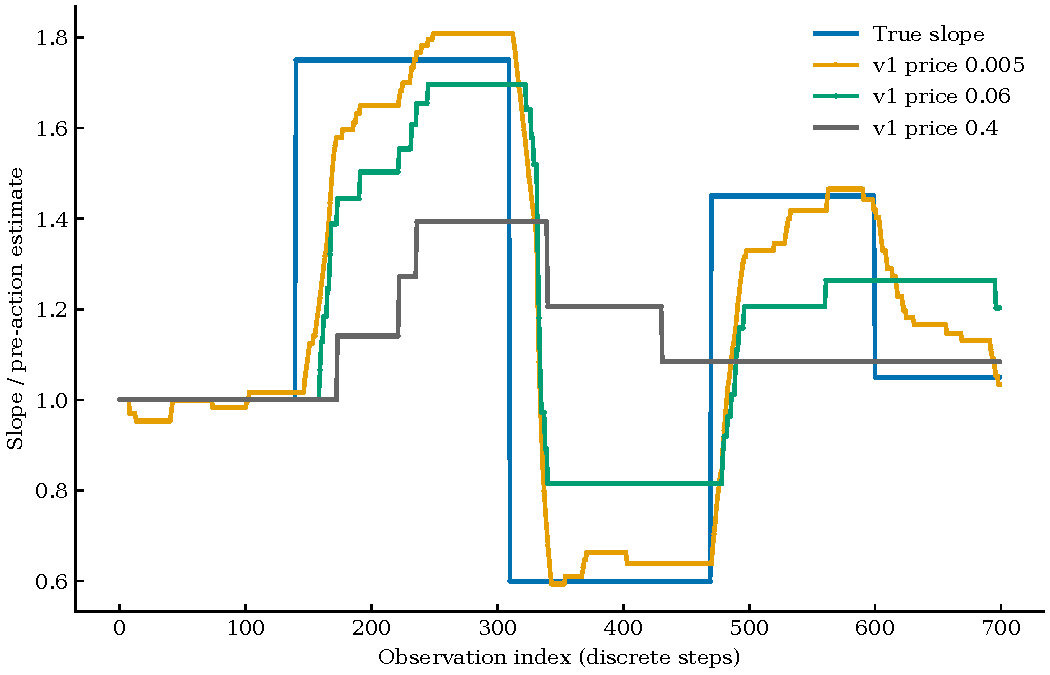
\includegraphics[width=0.88\textwidth]{figures/generated/slg-priced-policy-tracking-20261111.pdf}
\caption{Carried model state under actual-step pricing. The representative stream is seed 0, fixed before execution. The latent slope changes at observations \(140,310,470,600\) and is used only for evaluation. The other curves show the actual-step-priced rolling policy at the displayed prices. Each update moves \(0.22\) of the way towards the trailing ridge target and is bought only when \(2.5\) times its actual window improvement exceeds \(c\). Estimates are pre-action states. High prices can retain bias after a shift. This trace must be read with the matched risk, update-frequency and occupancy comparisons, not as a calibrated choice of price.}
\label{fig:num-toy-two-scale-promotion}
\end{figure*}

\subsection{Prediction risk is an external test}

Mean squared prediction error is evaluated over observations \(50,\ldots,699\), giving 650 predictions per stream. It is calculated before the current observation updates the model, rather than by rescoring the observation after fitting it. Figure~\ref{fig:prediction-risk} reports stream means at all six matched prices. The fixed-slope-1 baseline has mean error \(0.2899961\). A privileged predictor given the true slope has error \(0.0628541\), providing a noise-scale reference rather than an available policy.

The actual-step-priced policy has higher mean predictive error than the noisy-step policy at every tested matched price. At \(c=0.06\), their mean errors are approximately \(0.143405\) and \(0.121170\). The rolling control lies between them at \(0.129231\). Appendix~\ref{app:protocol} retains the full table. These observations rule out a predictive-dominance claim for this comparison. They do not contradict the action-accounting identity. That identity concerns the gain assigned to an executable candidate on an observed window, not the candidate's future predictive value.

\begin{figure*}[t]
\centering
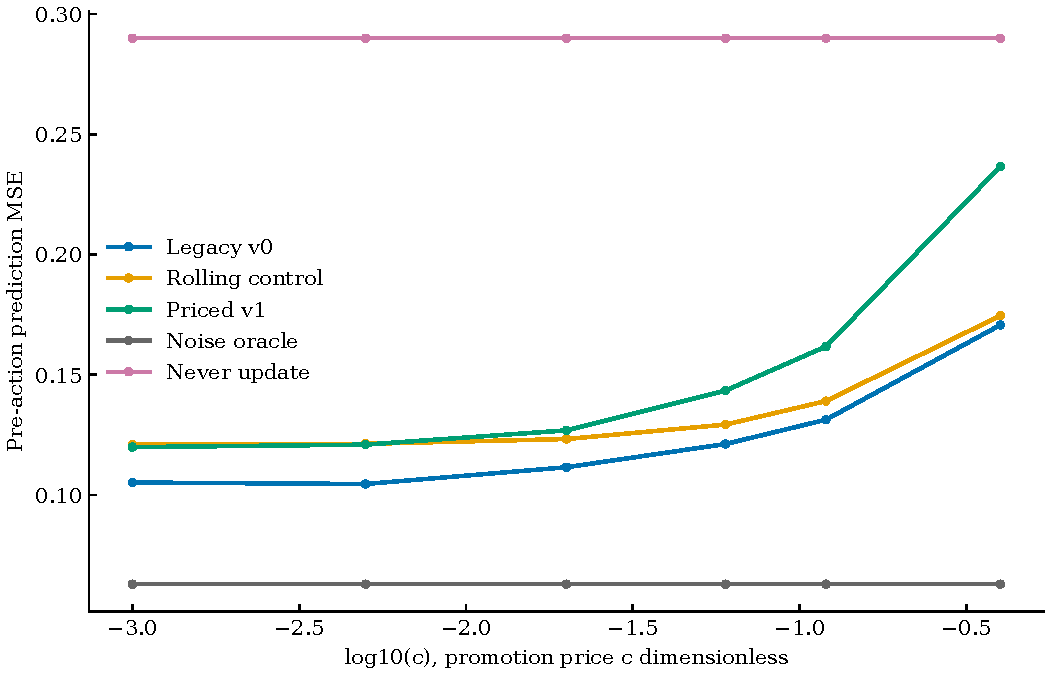
\includegraphics[width=0.84\textwidth]{figures/generated/slg-promotion-risk-20261111.pdf}
\caption{Prediction risk at matched prices. Mean squared one-step prediction error, in squared synthetic observation units, averaged over 12 matched 700-step streams using observations \(50\)--\(699\). The three methods are defined in the shared policy key in the text. The true-slope noise oracle is privileged and used only for evaluation. The never-update baseline keeps slope 1. Actual-step pricing has higher mean error than the noisy-step policy at every tested price. Lines connect the six predeclared finite stream means and carry no uncertainty bands. The complete means and the stream-level uncertainty convention are given in Appendix~\ref{app:protocol}.}
\label{fig:prediction-risk}
\end{figure*}

\subsection{Spending frequency does not measure adaptation}

The promotion fraction uses the same 650-observation window. Its numerator is the number of purchased model updates. The charged action cost per evaluated observation is \(c\) times this fraction. It does not include computation of candidates, controller maintenance or the cost of keeping a model in memory. It is a dimensionless accounting charge, not a measured energy consumption.

Figure~\ref{fig:promotion-frequency} shows the expected broad reduction in update frequency as price rises, but actual-step pricing is not always sparser than its comparators. At \(c=0.06\), the actual-step and noisy-step fractions are approximately \(0.050769\) and \(0.050385\). The actual-step policy therefore pays slightly more charged action cost while also having higher prediction error. At other prices it sometimes buys fewer updates while predicting worse. A sparse policy cannot be judged from its spending curve alone.

\begin{figure*}[t]
\centering
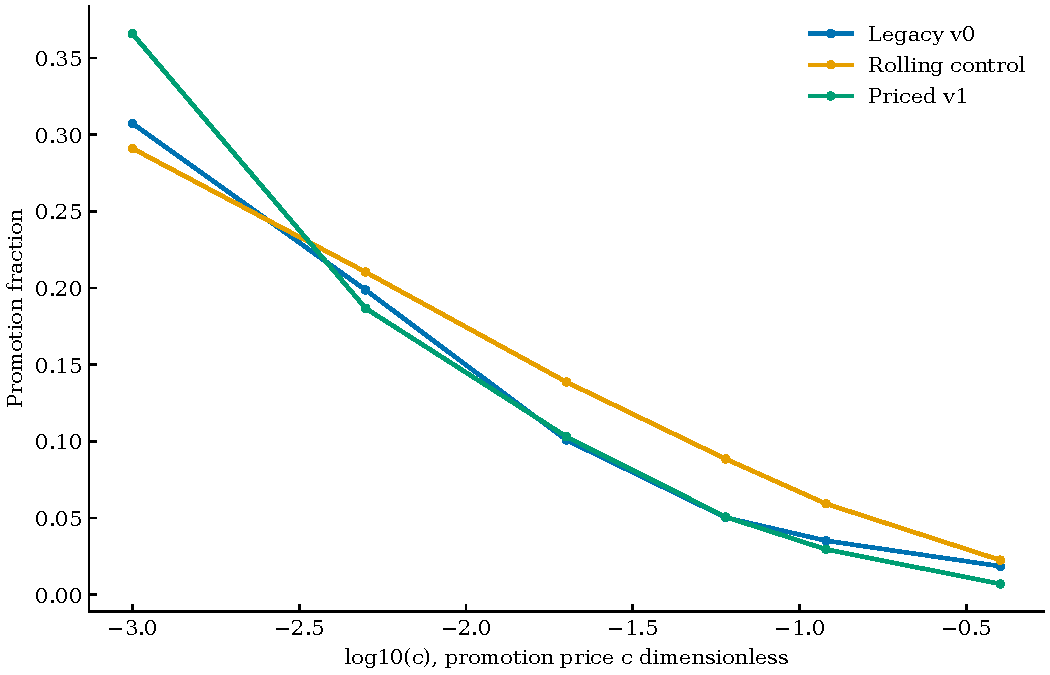
\includegraphics[width=0.84\textwidth]{figures/generated/slg-promotion-frequency-20261111.pdf}
\caption{How price changes update frequency. Promotion counts divided by 650 evaluated observations, averaged over the same 12 matched streams. Every promoted action pays the displayed dimensionless price \(c\), while staying pays zero action cost. Higher prices usually buy fewer revisions, but actual-step pricing is not always the sparsest policy. Multiplying a curve by \(c\) gives its charged action cost per evaluated observation, not total computational or physical cost. Read with Figs.~\ref{fig:prediction-risk} and \ref{fig:recovery}.}
\label{fig:promotion-frequency}
\end{figure*}

The target-occupancy test asks a different question. After a true shift, does the carried estimate enter and remain near the new target? A qualifying run consists of five consecutive pre-action estimates within \(20\%\) of the jump magnitude, entirely within the 65 observations beginning at the shift. An estimate already in band qualifies without any new update. Delay records the start of the run, not its confirmation four observations later. A shift with no qualifying run is assigned failure and a capped delay of 65.

Figure~\ref{fig:recovery} gives the fraction of shifts without such a run. Four shifts in 12 streams give 48 dependent shift evaluations per policy and price, not 48 independent experiments. At \(c=0.06\), failure fractions are \(0.1875\), \(0.270833\) and \(0.625\) for the noisy-step, rolling-control and actual-step-priced policies. Occupancy need not be monotone in price. A model that happens already to be near a later target can qualify even if it failed to react usefully to an earlier shift.

\begin{figure*}[t]
\centering
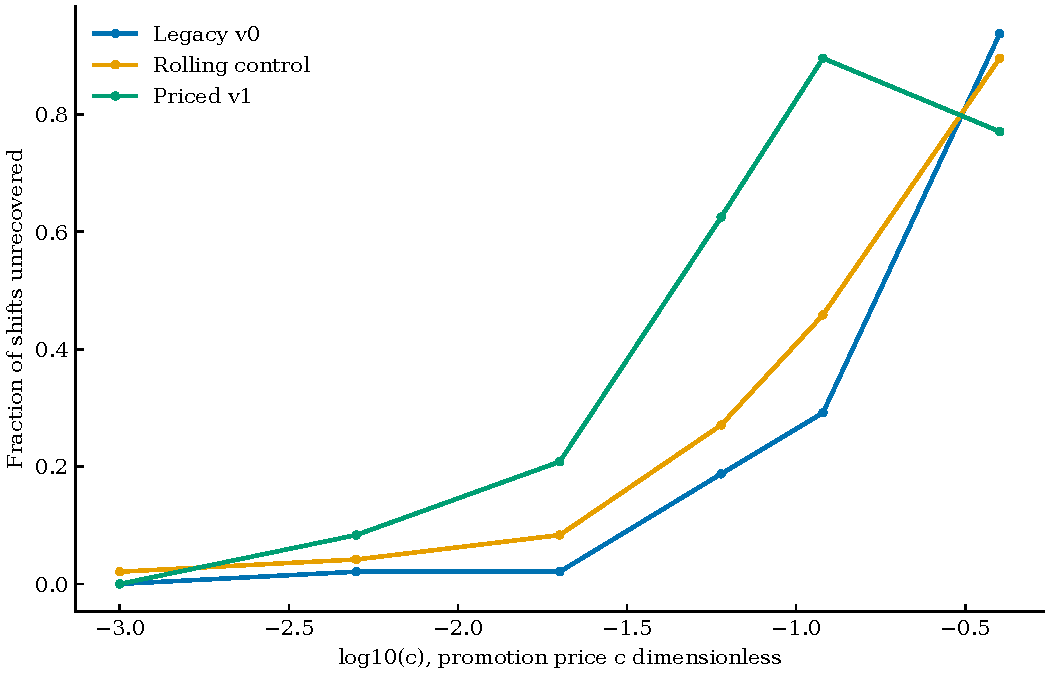
\includegraphics[width=0.84\textwidth]{figures/generated/slg-promotion-recovery-20261111.pdf}
\caption{Target occupancy after a latent shift. Fraction of shifts without five consecutive pre-action estimates in the declared band, averaged over 12 matched streams with four shifts each. The band is \(20\%\) of the jump magnitude, and the qualifying run must lie wholly within the 65-step post-shift window. Already-in-band estimates qualify without a new promotion. The criterion therefore measures occupancy, not detected change or update-caused recovery. Delay is the run start. Failures retain sentinel delay 65 in capped means. At \(c=0.06\), the three failure fractions are \(0.1875\), \(0.270833\) and \(0.625\). Lines are finite stream means without uncertainty bands.}
\label{fig:recovery}
\end{figure*}

The experiment exposes the remaining modelling task. Pricing the actual intervention prevents a mismatch between promised and executed gain. It does not tell us that an observed-window score is the right predictor of future benefit, or that a fixed price supplies adequate responsiveness after a shift. A better evaluator needs its own justified horizon, uncertainty model or parent signal. The finite results tell us where to improve the construction without discarding the accounting that makes the failure intelligible.

There is one more representational question. A receiver may not need every fine action or every step of a trace. It may ask only whether any revision occurred in a block. That is a smaller object than an adaptive trajectory. The next section derives exactly what it must retain, before asking whether a similarly small state can describe the full feedback process.
